%%%%%%%%%%%%%%%%%%%%%%%%%%%%%%%%%%%%%%%%%
% Beamer Presentation
% LaTeX Template
% Version 1.0 (10/11/12)
%
% This template has been downloaded from:
% http://www.LaTeXTemplates.com
%
% License:
% CC BY-NC-SA 3.0 (http://creativecommons.org/licenses/by-nc-sa/3.0/)
%
%%%%%%%%%%%%%%%%%%%%%%%%%%%%%%%%%%%%%%%%%

%------------------------------------------------------------------------------------------------
%   PACKAGES AND THEMES
%------------------------------------------------------------------------------------------------

\documentclass[table, xcolor = {dvipsnames}, 9pt]{beamer}
\usepackage{tikz}
\usetikzlibrary{backgrounds}
\usetikzlibrary{arrows,shapes}
\usetikzlibrary{tikzmark}
\usetikzlibrary{calc}
\usetikzlibrary{colorbrewer}
\mode<presentation> {

% The Beamer class comes with a number of default slide themes
% which change the colors and layouts of slides. Below this is a list
% of all the themes, uncomment each in turn to see what they look like.

\usetheme{default}
%\usetheme{AnnArbor}
%\usetheme{Antibes}
%\usetheme{Bergen}
%\usetheme{Berkeley}
%\usetheme{Berlin}
%\usetheme{Boadilla}
%\usetheme{CambridgeUS}
%\usetheme{Copenhagen}
%\usetheme{Darmstadt}
%\usetheme{Dresden}
%\usetheme{Frankfurt}
%\usetheme{Goettingen}
%\usetheme{Hannover}
%\usetheme{Ilmenau}
%\usetheme{JuanLesPins}
%\usetheme{Luebeck}
%\usetheme{Madrid}
\usetheme{metropolis}
%\usetheme{Malmoe}
%\usetheme{Marburg}
%\usetheme{Montpellier}
%\usetheme{PaloAlto}
%\usetheme{Pittsburgh}
%\usetheme{Rochester}
%\usetheme{Singapore}
%\usetheme{Szeged}
%\usetheme{Warsaw}

% As well as themes, the Beamer class has a number of color themes
% for any slide theme. Uncomment each of these in turn to see how it
% changes the colors of your current slide theme.

%\usecolortheme{albatross}
%\usecolortheme{beaver}
%\usecolortheme{beetle}
%\usecolortheme{crane}
%\usecolortheme{dolphin}
%\usecolortheme{dove}
%\usecolortheme{fly}
%\usecolortheme{lily}
%\usecolortheme{orchid}
%\usecolortheme{rose}
\usecolortheme{seagull}
%\usecolortheme{seahorse}
%\usecolortheme{whale}
%\usecolortheme{wolverine}
\usefonttheme{professionalfonts}
%\setbeamertemplate{footline} % To remove the footer line in all slides uncomment this line
%\setbeamertemplate{footline}[page number] % To replace the footer line in all slides with a simple slide count uncomment this line

%\setbeamertemplate{navigation symbols}{} % To remove the navigation symbols from the bottom of all slides uncomment this line
}

\usepackage{graphicx} % Allows including images
\usepackage{booktabs} % Allows the use of \toprule, \givenrule and \bottomrule in tables
\usepackage{multirow}
\usepackage{xspace}
\usepackage{natbib}
\usepackage{hyperref}
\usepackage{diagbox}
\usepackage{makecell}
\usepackage{xparse}
\usepackage{subfig}
\usepackage{amsfonts,amsthm,amsmath,amssymb}
\usepackage{mathtools, nccmath}
\usepackage[ruled, vlined, linesnumbered]{algorithm2e}
\usepackage{wrapfig}
\usepackage{comment}  
\usepackage{bbm}
\usepackage{bm}
\usepackage{empheq}
\usepackage{pgfplots}
\usepgfplotslibrary{colorbrewer}
\usepackage{animate}
\usepackage{array}
\usepackage{ragged2e}
\newcolumntype{P}[1]{>{\RaggedRight\hspace{0pt}}p{#1}}
\newcolumntype{X}[1]{>{\RaggedRight\hspace*{0pt}}p{#1}}

% color box
\usepackage{tcolorbox}
\usepackage{tikz}
\usetikzlibrary{backgrounds}
\usetikzlibrary{arrows,shapes}
\usetikzlibrary{tikzmark}
\usetikzlibrary{calc}
% Commands for Highlighting text -- non tikz method
\newcommand{\highlight}[2]{\colorbox{#1!17}{$\displaystyle #2$}}
%\newcommand{\highlight}[2]{\colorbox{#1!17}{$#2$}}
\newcommand{\highlightdark}[2]{\colorbox{#1!47}{$\displaystyle #2$}}

% my custom colors for shading
\colorlet{mhpurple}{Plum!80}


% Commands for Highlighting text -- non tikz method
\renewcommand{\highlight}[2]{\colorbox{#1!17}{#2}}
\renewcommand{\highlightdark}[2]{\colorbox{#1!47}{#2}}

\usepgfplotslibrary{colorbrewer}

\newcommand\mybox[2][]{\tikz[overlay]\node[fill=lightgray,inner sep=2pt, anchor=text, rectangle, rounded corners=1mm,#1] {#2};\phantom{#2}}
\hypersetup{unicode=true,
            bookmarksnumbered=true,
            bookmarksopen=true,
            bookmarksopenlevel=2,
            breaklinks=false,
            pdfborder={0 0 1},
            hypertexnames=false,
            pdfstartview={XYZ null null 1}}
\usepackage{xcolor}
\hypersetup{
    colorlinks,
    linkcolor={red!50!black},
    citecolor={blue!50!black},
    urlcolor={blue!80!black}
}
\newcommand\myheading[1]{%
  \par\bigskip
  {\Large\bfseries#1}\par\smallskip}
\newcommand\given[1][]{\:#1\vert\:}
\theoremstyle{plain}
\newtheorem{thm}{Theorem}
\newtheorem{prop}{Proposition\thisthmnumber}
\newtheorem{lem}{Lemma\thisthmnumber}
\newtheorem{cor}{Corollary}
\newtheorem{defin}{Definition}
\newtheorem{algo}{Algorithm}
\newcommand*\diff{\mathop{}\!\mathrm{d}}
\newcommand*\Diff[1]{\mathop{}\!\mathrm{d^#1}}
\newcommand{\thisthmnumber}{}
\newcommand*{\QEDA}{\hfill\ensuremath{\blacksquare}}%
\newcommand*{\QEDB}{\hfill\ensuremath{\square}}%
\newcommand{\norm}[1]{\left\lVert#1\right\rVert}
\DeclareMathOperator{\N}{\mathbb{N}}
\DeclareMathOperator{\E}{\rm{E}}
\DeclareMathOperator{\R}{\mathbb{R}}
\DeclareMathOperator{\Var}{\rm{Var}}
\DeclareMathOperator{\Cov}{\rm{Cov}}
\DeclareMathOperator{\e}{\rm{e}}
\DeclareMathOperator{\logit}{\rm{logit}}
\DeclareMathOperator{\indep}{{\perp\!\!\!\perp}}
\DeclareMathOperator{\rank}{rank}
\DeclareMathOperator*{\argmin}{arg\,min}
\DeclareMathOperator*{\argmax}{arg\,max}
%\DeclareMathOperator{\Pr}{\rm{Pr}}
%------------------------------------------------------------------------
%	TITLE PAGE
%-----------------------------------------------------------------------
\pagestyle{empty}
\title[]{Introduction to observational studies} % The short title appears at the bottom of every slide, the full title is only on the title page

\author{Thomas Leavitt and Ben Hansen} 
\institute[]
{

}
\date{June 26, 2024} 

\NewDocumentEnvironment{statement}{mo}
 {%
  \IfValueT{#2}{\renewcommand{\thisthmnumber}{ #2}}\begin{#1}%
 }
 {\end{#1}}

\begin{document}

\begin{frame}
\titlepage % Print the title page as the first slide
\end{frame}

%\begin{frame}
%\frametitle{Overview} % Table of contents slide, comment this block out to remove it
%\tableofcontents % Throughout your presentation, if you choose to use \section{} and \subsection{} commands, these will automatically be printed on this slide as an overview of your presentation
%\end{frame}

%-------------------------------------------------------------------------------------
%	PRESENTATION SLIDES
%-------------------------------------------------------------------------------------
\section{Review: Randomized Experiments}
\begin{frame}[t]
\frametitle{Randomized experiments}
\vfill
\begin{itemize} \vfill
\item \textbf{Treatment}: $z_i$ is indicator of treatment for unit $i$, where $i = 1, \ldots, N$ \vfill
\begin{itemize} \vfill
\item The subscript $i$ is a placeholder referring to arbitrary unit \vfill
\item E.g., $z_5$ is the treatment indicator for the $5$th unit \vfill
\end{itemize} \vfill
\begin{align*}
z_i & = 
\begin{cases}
1 & \text{if unit } i \text{ assigned to treatment} \\
0 & \text{otherwise}
\end{cases}
\end{align*} \vfill
\item In randomized controlled trial, \vfill 
\item[] each subject assigned to treatment and control via \textcolor{magenta}{known}, \textcolor{magenta}{chance} process \vfill
\begin{itemize} \vfill
\item E.g., if we flip a fair coin for each unit, probability of treatment assignment is $0.5$ for all units; $\Pr\left(Z_i = 1\right) = 0.5$ for all $i$
\end{itemize} \vfill
\end{itemize}
\vfill
\end{frame}
%-------------------------------------------------------------------------------------
\begin{frame}[t]
\frametitle{Randomized experiments}
\vfill
\begin{itemize} \vfill
\item Randomization $\implies$ \vfill
\item[] procedure for generating estimates of ATE will be correct, on average \vfill
\item Randomization is foundation for valid hypothesis tests about causal effects \vfill
\begin{itemize} \vfill
\item The ``reasoned basis'' for inference \small \citep[][p.~14]{fisher1935a} \normalsize \vfill
\end{itemize} \vfill
\end{itemize}
\vfill
\end{frame}
%-------------------------------------------------------------------------------------
\section{Observational studies}
\begin{frame}[t]
\frametitle{Observational studies}
\vfill
\begin{itemize} \vfill
\item Observational study: \vfill
\item[] Empirical investigation in which ``it is not feasible to use controlled experimentation in the sense of being able to ... assign subjects at random to different procedures'' \citep{cochran1965} \vfill
\item In observational study, subjects \textcolor{magenta}{select} into treatment and control conditions via \textcolor{magenta}{unknown}, \textcolor{magenta}{chance} process \vfill
\begin{itemize} \vfill
\item Think of this as \\ ``assignment to treatment group on the basis of a covariate'' \citep{rubin1977} \vfill
\end{itemize} \vfill
\end{itemize}
\vfill
\end{frame}
%-------------------------------------------------------------------------------------
\begin{frame}[t]
\frametitle{Observational studies}
\vfill
\begin{itemize} \vfill
\item In observational study, subjects \textcolor{magenta}{select} into treatment and control conditions via \textcolor{magenta}{unknown}, \textcolor{magenta}{chance} process \vfill
\item \textcolor{magenta}{Propensity score} \vfill
\item[] Probability of selecting into treatment as a function of baseline covariates \vfill
\begin{itemize} \vfill
\item Propensity scores are \textcolor{magenta}{unknown} and cannot be directly measured \vfill
\item In principle, baseline covariates that determine treatment assignment probabilities can be measured \vfill
\end{itemize} \vfill
\end{itemize} \vfill
\end{frame}
%-------------------------------------------------------------------------------------
\begin{frame}[t]
\frametitle{Observational studies}
\vfill
Model of an observational study \citep{rosenbaum2002a} \vfill
\begin{itemize} \vfill
\item \textcolor{magenta}{Independent} but not necessarily \textcolor{magenta}{identically} distributed assignments \vfill
\begin{align} \label{eq: obs study mod}
\Pr\left(\bm{Z} = \bm{z}\right) = \prod \limits_{i = 1}^N \pi_i^{z_i} (1 - \pi_i)^{1 - z_i},
\end{align}
where $\pi_i \in [0, 1]$ is probability of treatment \vfill
\item \textcolor{magenta}{Propensity score} \vfill
\item For each unit, $\pi_i$ is function of covariates, either observed, $\bm{x}_i$, or unobserved, $\bm{u}_i$ \vfill
\begin{itemize} \vfill
\item Under \textcolor{magenta}{no hidden bias}, $\pi_i = \lambda(\bm{x}_i)$, where $\lambda$ is a function, $\lambda: \R^K \mapsto [0, 1]$, whose form is unknown \vfill
\item Under \textcolor{magenta}{common support}, $\pi \in (0, 1)$ for all $i = 1, \ldots , N$ \vfill
\end{itemize} \vfill
\end{itemize} \vfill
\end{frame}
%-------------------------------------------------------------------------------------
\begin{frame}[t]
\frametitle{Observational studies}
\vfill
\begin{itemize} \vfill
\item We want to compare ``apples to apples,'' \textit{not} ``apples to oranges'' \\ \citep{rubinwaterman2006} \vfill
\begin{itemize} \vfill
\item I.e., make strata of treated and control units \textcolor{magenta}{homogeneous in propensity scores} \vfill
\end{itemize} \vfill
\item Although propensity scores unknown, if any two units are same on covariates that determine treatment assignment probability \vfill
\item[] $\implies$ identical propensity scores \vfill
\end{itemize} \vfill
\end{frame}
%-------------------------------------------------------------------------------------
\begin{frame}[t]
\frametitle{Observational studies}
\vfill
\begin{itemize} \vfill
\item If we can justify we are comparing treated and control units with \textcolor{magenta}{same} propensity scores \vfill
\item[] $\rightarrow$ Then act as if we have mini randomized experiment within each block \vfill
\item We do \textbf{not} need to know units' true propensity scores \vfill
\item We need to justify only that propensity scores are the \textcolor{magenta}{same} within blocks \vfill
\begin{itemize} \vfill
\item E.g., in block A with one treated and one control unit, it does not matter if propensity scores are $0.7$ and $0.7$; $0.2$ and $0.2$; or any other values \vfill
\end{itemize} \vfill
\end{itemize} \vfill
\end{frame}
%-------------------------------------------------------------------------------------
\begin{frame}[t]
\frametitle{Observational studies}
\vfill
\begin{itemize} \vfill
\item More formally, let $s = 1, \ldots , S$ tun over $S$ strata \vfill
\item If $\pi_{s,i} = \pi_{s,j}$ for all $i,j = 1, \ldots , n_s$ in stratum $s$, then \vfill 
\begin{align*}
\Pr\left(\bm{Z}_z = \bm{z}_s\right) = \dfrac{1}{\left\lvert \Omega_s \right\rvert} \text{ for all } \bm{z}_s \in \Omega_s, \text{ where } \Omega_s = \left\{\bm{z}_s: \sum \limits_{i = 1}^{n_s} z_{s,i} = n_{1,s}\right\}
\end{align*} \vfill
\item[$\star$] As-if randomization holds conditional on observed number of treated units \vfill
\end{itemize} \vfill
\end{frame}
%-------------------------------------------------------------------------------------
\begin{frame}[t]
\frametitle{Observational studies}
\vfill
\begin{itemize} \vfill
\item E.g., stratum with $3$ units, $1$ treated and $2$ control, all with propensity score of $0.35$ \vfill
\item Without conditioning on $1$ treated unit, model in \eqref{eq: obs study mod} yields \vfill
\small
\begin{align*}
\Pr\left(\bm{Z}_s = \begin{bmatrix} 0 & 0 & 0 \end{bmatrix}^{\top}\right) & = (1 - 0.35) (1 - 0.35) (1 - 0.35) = 0.274625 \\
\Pr\left(\bm{Z}_s = \begin{bmatrix} 0 & 0 & 1 \end{bmatrix}^{\top}\right) & = (1 - 0.35) (1 - 0.35) (0.35) = 0.147875 \\
\Pr\left(\bm{Z}_s = \begin{bmatrix} 0 & 1 & 0 \end{bmatrix}^{\top}\right) & = (1 - 0.35) (0.35) (1 - 0.35) = 0.147875 \\
\Pr\left(\bm{Z}_s = \begin{bmatrix} 1 & 0 & 0 \end{bmatrix}^{\top}\right) & = (0.35) (1 - 0.35) (1 - 0.35) = 0.147875 \\
\Pr\left(\bm{Z}_s = \begin{bmatrix} 0 & 1 & 1 \end{bmatrix}^{\top}\right) & = (1 - 0.35) (0.35) (0.35) = 0.079625 \\
\Pr\left(\bm{Z}_s = \begin{bmatrix} 1 & 0 & 1 \end{bmatrix}^{\top}\right) & = (0.35) (1 - 0.35) (0.35) = 0.079625 \\
\Pr\left(\bm{Z}_s = \begin{bmatrix} 1 & 1 & 0 \end{bmatrix}^{\top}\right) & = (0.35) (0.35) (1 - 0.35) = 0.079625 \\
\Pr\left(\bm{Z}_s = \begin{bmatrix} 1 & 1 & 1 \end{bmatrix}^{\top}\right) & = (0.35) (0.35) (0.35) = 0.042875 \\
\end{align*}
\normalsize \vfill
\end{itemize} \vfill
\end{frame}
%-------------------------------------------------------------------------------------
\begin{frame}[t]
\frametitle{Observational studies}
\vfill
\begin{itemize} \vfill
\item With conditioning on $1$ treated unit, model in \eqref{eq: obs study mod} and def.~of conditional probability yield \vfill
\small
\begin{align*}
\Pr\left(\bm{Z}_s = \begin{bmatrix} 0 & 0 & 1 \end{bmatrix}^{\top}\right) & = 0.147875 \, / \, [(0.147875)(3)] = 1/3 \\
\Pr\left(\bm{Z}_s = \begin{bmatrix} 0 & 1 & 0 \end{bmatrix}^{\top}\right) & = 0.147875 \, / \, [(0.147875)(3)] = 1/3 \\
\Pr\left(\bm{Z}_s = \begin{bmatrix} 1 & 0 & 0 \end{bmatrix}^{\top}\right) & = 0.147875 \, / \, [(0.147875)(3)] = 1/3
\end{align*}
\normalsize \vfill
\item We now have uniform distribution on $\Omega_s$ \vfill 
\item[] I.e., completely randomized experiment within stratum $s$ \vfill
\end{itemize} \vfill
\end{frame}
%-------------------------------------------------------------------------------------
\begin{frame}[t]
\frametitle{Observational studies}
\vfill
\textcolor{magenta}{Two concerns} \vfill
\begin{itemize} \vfill
\item In practice, even under no hidden bias, exact stratification on covariates determining assignment probabilities is difficult or impossible \vfill
\begin{itemize} \vfill
\item[$\star$] Exact stratification on covariates \textbf{sufficient}, but not \textbf{necessary}, for homogeneous assignment probabilities within strata \vfill
\item Common instead to stratify on \textbf{estimated} propensity score \vfill
\end{itemize} \vfill
\item Propensity scores may differ within strata due to unobserved covariates, $\bm{u}$ \vfill
\end{itemize} \vfill
We will address both concerns in days on matching and sensitivity analysis
\end{frame}
%-------------------------------------------------------------------------------------
\section{Estimation and testing}
\begin{frame}[t]
\frametitle{Estimation and testing}
\vfill
\begin{itemize} \vfill
\item Create strata of similar units (in their unobservable propensity scores) \vfill
\item Then estimate ATE or test hypotheses about effects \textcolor{magenta}{within blocks}
\begin{itemize} \vfill
\item Act as-if we have a mini randomized experiment within blocks \vfill
\end{itemize} \vfill
\item Overall estimate or test then averages over results in all mini-experiments \vfill
\end{itemize}
\vfill 
\end{frame}
%-------------------------------------------------------------------------------------
\begin{frame}[t]
\frametitle{Example: Estimation and testing}
\vfill
\begin{itemize} \vfill
\item \citet[][p.~66-70]{rosenbaum2017} \vfill
\begin{itemize} \vfill
\item Treatment vs.~control comparison \vfill
\item Outcome: mortality \vfill
\item Two covariates \vfill
\begin{itemize} \vfill
\item age (young or old) \vfill
\item sex (male or female) \vfill
\end{itemize} \vfill
\item Probability of treatment for young men and young women $= 0.2$ \vfill
\item Probability of treatment for old men and old women $= 0.8$ \vfill
\end{itemize} \vfill
\end{itemize}  
\vfill 
\end{frame}
%-------------------------------------------------------------------------------------
\begin{frame}[t]
\frametitle{Example: Estimation and testing}
\vfill
\begin{figure}
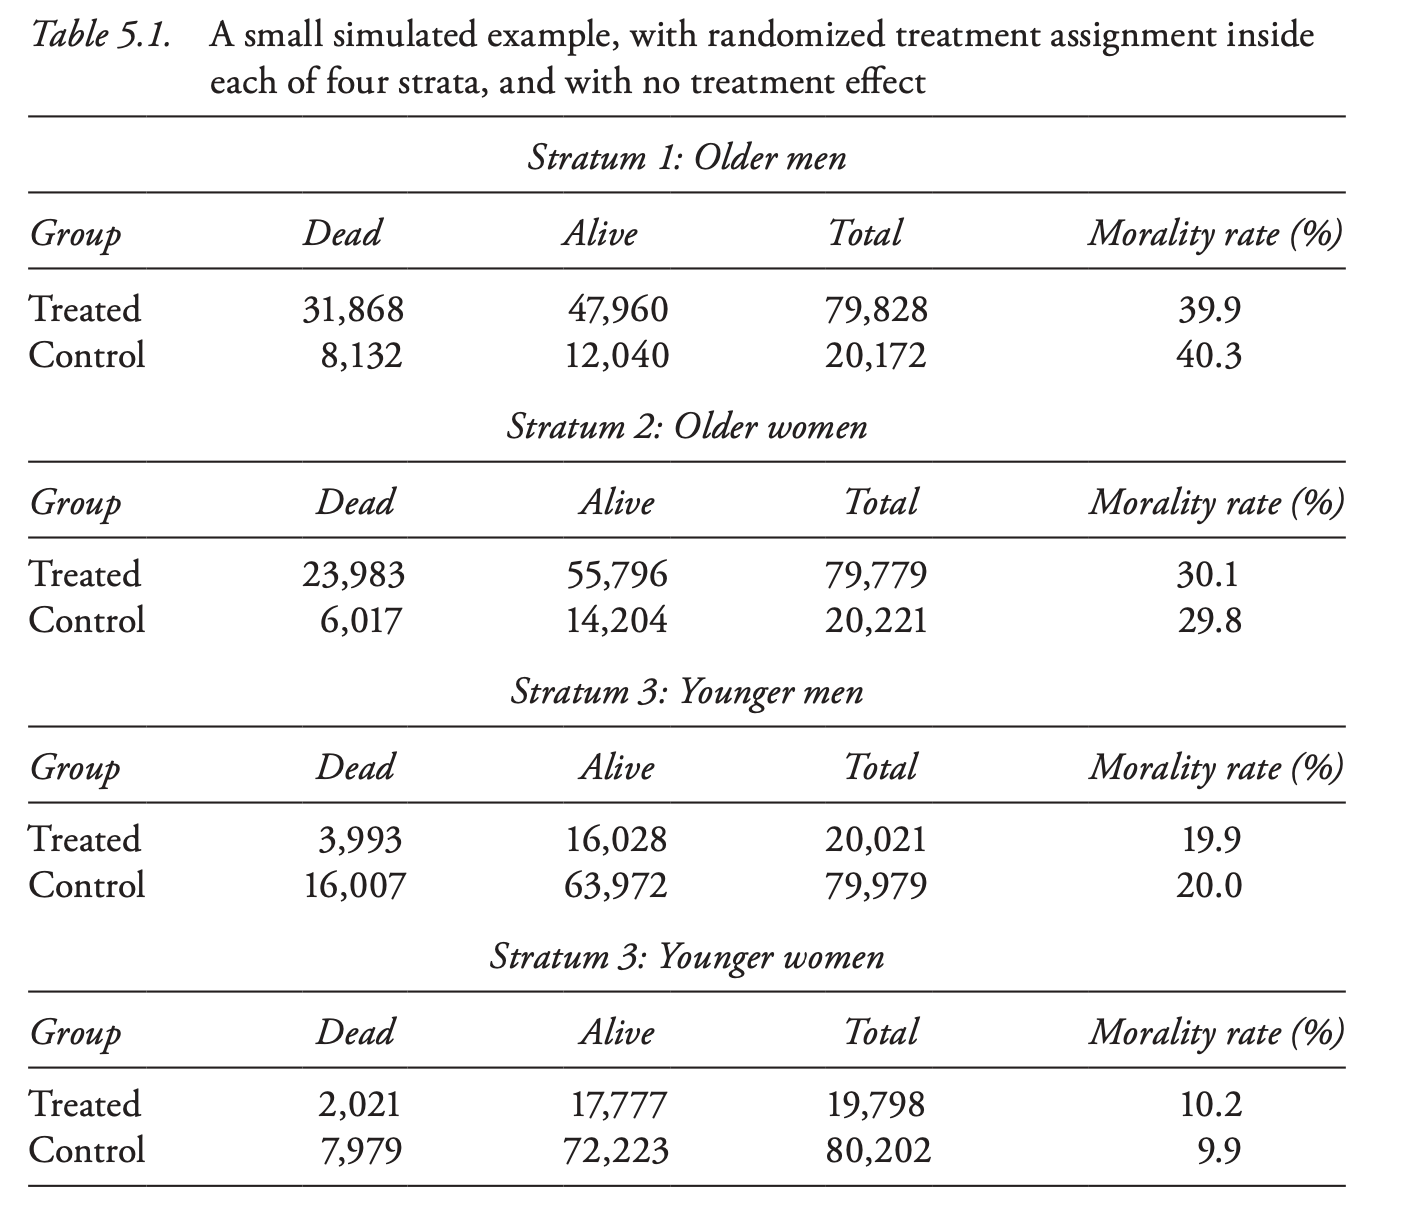
\includegraphics[width = 0.8\linewidth]{figures/Rosenbaum_2017_Table_5.1.png}
\caption{\citep[][p.~67]{rosenbaum2017}}
\end{figure}
\vfill 
\end{frame}
%-------------------------------------------------------------------------------------
\begin{frame}[t]
\frametitle{Example: Estimation and testing}
\vfill
\begin{figure}
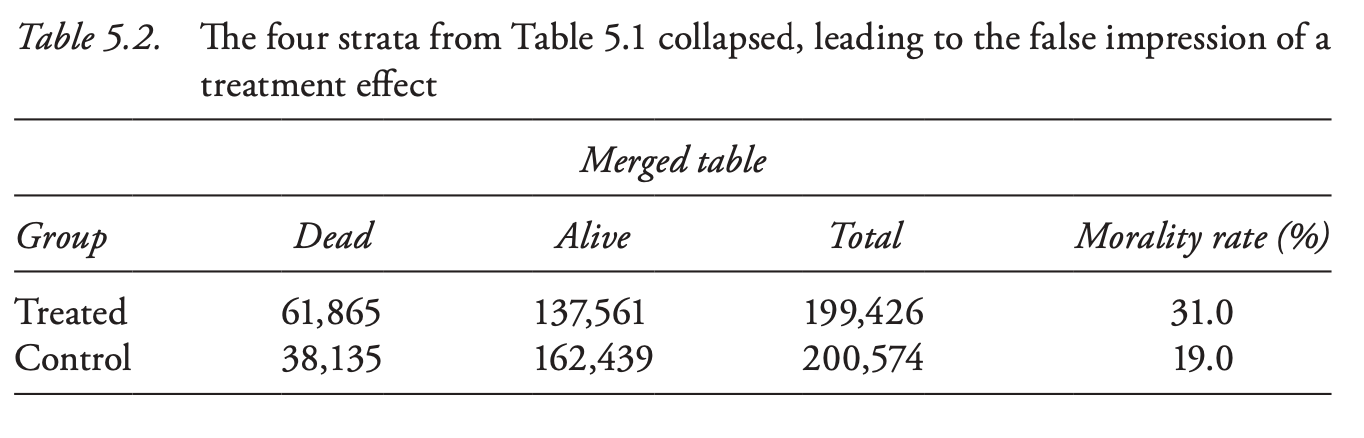
\includegraphics[width = \linewidth]{figures/Rosenbaum_2017_Table_5.2.png}
\caption{\citep[][p.~69]{rosenbaum2017}}
\end{figure}
\vfill 
\begin{itemize} \vfill
\item Older people more likely to be treated (prob $= 0.8$) \vfill
\item Older people also have greater baseline mortality rate \vfill
\item[$\implies$]  treated group composed mainly of older people \vfill
\item[] and control group composed mainly of younger people \vfill
\item[$\implies$] appears to be an effect when there is none \vfill
\end{itemize} \vfill 
\end{frame}
%-------------------------------------------------------------------------------------
\begin{frame}[allowframebreaks]
\frametitle{References} 
\scriptsize
\bibliographystyle{chicago}
\bibliography{Bibliography.bib}   % name your BibTeX data base
\end{frame}
%-------------------------------------------------------------------------------------
\end{document}